\begin{refsection}

\hypertarget{patterns-of-co-occurrence-and-spatial-richness-in-marine-habitats-insights-from-large-scale-modelling}{%
\chapter{Patterns of Co-occurrence and Spatial Richness in Marine
Habitats: Insights from Large-Scale
Modelling}\label{patterns-of-co-occurrence-and-spatial-richness-in-marine-habitats-insights-from-large-scale-modelling}}

\hypertarget{preambule-chapter3}{%
\section*{Préambule}\label{preambule-chapter3}}
\addcontentsline{toc}{section}{Préambule}

Grâce au Chapitre 2, nous avons identifié différents états d'habitats
biogéniques à l'échelle mondiale en appliquant une nouvelle méthode
d'agrégation que nous avons appliquée à des données d'un programme de
sciences participatives. Maintenant que les états d'habitats ont été
définis, ce chapitre vise à modéliser leur distribution à l'aide d'une
approche spatiale semblable à celle utilisée dans le cadre des
\emph{SDM}. Nous avons choisi de recentrer ces analyses du Chapitre 3
sur la région australo-pacifique, cœur géographique historique du
programme \emph{Reef Life Survey} \autocite{Edgar_2009}. L'objectif
premier est de comprendre les facteurs environnementaux et anthropiques
influençant leurs occurrences. En caractérisant les niches
environnementales, un second objectif est de déterminer les habitats
partageant des niches similaires donc susceptibles de coexister le long
des côtes australiennes. Dans ce contexte, ce chapitre vise à étudier la
distribution de 14 états d'habitats sur les côtes australiennes.

Nous avons utilisé un \emph{SDM} de type \emph{Random Forest} multivarié
pour caractériser les niches environnementales des états d'habitats en
considérant comme prédicteurs des données environnementales
(\emph{Bio-Oracle}; \textcite{Assis_2018}), et des données de pressions
anthropiques (\emph{Ocean Health Index} ; \textcite{Halpern_2019}). Nos
résultats indiquent que le modèle a un bon pouvoir explicatif, mais un
pouvoir prédictif faible, laissant penser que la transférabilité de
notre modèle dans le temps et l'espace est restreinte. Nos résultats
indiquent que les facteurs les plus importants régissant la distribution
de ces différents états d'habitats sont la température de surface de
l'eau, l'intensité de la pression de pêche et les anomalies dans la
fréquence des vagues de chaleur marine. Nous montrons également dans ce
chapitre que tous les états d'habitat identifiés ne pouvaient co-exister
dans le même transect ce qui suggère que certaines combinaisons d'états
d'habitats sont invraisemblables (ou jamais observées à ce jour). Ce
travail a permis également de mettre en avant que les zones de
transitions tempérées/tropicales sont susceptibles d' abriter un plus
grand nombre d'états d'habitats. Cela peut impliquer que ces zones sont
plus exposées aux changements de régime, puisque la disparition de
l'état dominant actuel pourrait laisser place au développement d'un état
d'habitat différent, notamment dans un contexte de tropicalisation des
zones tempérées chaudes des côtes est \autocites[
]{Verges_2014}{Verges_2019} et ouest \autocite{Wernberg_2016}
australiennes. Ces changements sont d'autant plus importants à
surveiller puisqu'ils pourraient avoir un impact important sur la
composition et les fonctions des communautés associées et par conséquent
modifier le fonctionnement même des écosystèmes.

Ce chapitre de thèse est l'oeuvre de la collaboration de Clément Violet, Aurélien Boyé, Mathieu Chevalier et de Martin Marzloff.

\clearpage

\hypertarget{abstract-chapt3}{%
\section{Abstract}\label{abstract-chapt3}}

Benthic reef habitats serve as foundational structures in coastal
ecosystems, facilitating essential ecological processes and
significantly amplifying biodiversity. However they are increasingly
subject to regime shifts that can be detrimental for marine ecosystem
functioning and biodiversity. In this study we aim to investigate the
distribution and ecological drivers of reef benthic habitat states
across Australia, in order to understand and anticipate their
potential/risk of ecological regime shifts in the face of changing
environments and anthropogenic impacts. Using random forest models
applied to occurrences of reef habitat states stemming from a previous
analyses of the \emph{Reef Life Survey} transect data, we quantified the
relative contribution of anthropogenic and environmental drivers in
explaining their spatial distribution. Specifically, we focused on 14
reef states including turf, kelp or coral reefs. Models showed a good
explanatory power with AUC (\(\text{mean} = 0.87\);
\(\text{sd} = 0.07\)). For most habitats, we found that SST, Fishing
intensity and Marine Heatwaves were the most important driver of their
distribution while anthropogenic factors only had a marginal influence.
However, models presented a poor predictive power suggesting limited
transferability in time or space. On the calibration areas, we found
that several habitats (up to eight) can occur under similar
environmental conditions, suggesting that the likelihood of state
changes (including regime shifts) is spatially variable. Overall, this
approach makes it possible to highlight areas and environmental
conditions where the occurrence of alternative stable states is more
likely.

\clearpage

\hypertarget{intro-chapt3}{%
\section{Introduction}\label{intro-chapt3}}

Regime shifts are persistent changes in the structure and/or the
function of ecosystems occurring more or less suddenly \autocites[
]{Scheffer_2001}{Scheffer_2003}. Ecological regime shifts have been
identified in many different ecosystems: forest to savannahs
\autocite{Staver_2011}, tundra to boreal forests
\autocite{Scheffer_2012}, coral reefs to macroalgae dominated reefs
\autocite{McManus_2004}, or fisheries collapse \autocite{Gardmark_2015}.
Areas affected by regime shifts tend usually display profound and
lasting changes in the ecosystem services they provide to human
populations \autocite{Rocha_2015a}, with economic impacts through the
disappearance of certain activities \autocite{Crepin_2012}, and societal
and cultural impacts through the loss of cultural and traditional
knowledge \autocite{Mustonen_2021}. Thus, one of the common features of
all these regime shifts is that they drive the ecosystem under
consideration towards a new state, considered from a human perspective
to be less desirable \autocite{Scheffer_2009bk}.

Multiple factors can trigger a change in ecological regime towards a new
ecosystem states \autocite{Rocha_2015b}. These factors include climatic
variations caused by global climate change \autocite{Rocha_2015b},
increase in the number of extreme climatic events
\autocite{Wernberg_2016}, introduction of invasive species
\autocite{Kotta_2018}, increase in anthropogenic pressure
\autocite{Halpern_2019}, and loss of biogenic habitats
\autocite{Airoldi_2008}.

Biogenic habitats, formed by engineers' species, play a crucial role in
the functioning of marine coastal ecosystems and in supporting
components of biodiversity \autocites[ ]{Vozzo_2023}{Albertson_2022}.
For instance, mangroves serve as a nursery for coral-reef fish
\autocite{Nagelkerken_2002}, coral act as a refuge from predators for
many fish and invertebrates species \autocite{Almany_2004}, marine
seagrasses enhance water quality by for instance increasing water pH
\autocite{Ricart_2021}, and their presence increases infauna diversity
\autocites[ ]{Gonzalez-Ortiz_2016}{Boye_2017}. Because biogenic habitats
are also vulnerable to human pressures and natural disturbances
\autocites[ ]{Airoldi_2007}[ ]{Butt_2022}{Wernberg_2023}, they play a
central role in mediating the effects of current environmental changes
on marine coastal ecosystems and biodiversity \autocites[
]{Sunday_2017}{Bulleri_2018}.

Over the last few decades, regime shifts involving persistent changes in
biogenic benthic habitats have been observed worldwide across temperate
and tropical regions. Examples include shifts from macroalgal forests to
either sea urchin barrens \autocite{Ling_2015} or turf
\autocite{Filbee-Dexter_2018}, from crustose coralline algae to turf
\autocite{Cornwall_2023}, and also from coral-dominated reefs to
macroalgae \autocite{McManus_2004}, or from seagrass to bare sediments
\autocite{Maxwell_2017}. These regime shifts share in common that as the
biogenic habitats degrade or change, novel ecological dynamics take root
to push and maintain the ecosystems into new states
\autocite{Nystrom_2012}. As these new states are often undesirable from
a management perspective while also displaying hysteresis making it
difficult to return to the initial state \autocite{Nystrom_2012},
substantial efforts have been devoted to identifying, predicting and
preventing regime shifts before they occur \autocite{Biggs_2009}.
Detection of early warning signals of regime shifts has been intensively
investigated by analysing temporal ecosystem dynamics when long-term
time series are available \autocite{Scheffer_2009}, or spatial patterns
emerging from ecological dynamics \autocites[ ]{Kefi_2014}[
]{Nijp_2019}{Ward_2018}. Although promising theoretically based on
numerical or mesocosm experiments, these data-greedy methods remain of
limited practical interest in real world ecosystems across large spatial
scales , as (i) they are often computed retrospectively after the shift
has occurred (e.g. \textcite{Litzow_2014}) and (ii) to date, no single
metrics amongst the alternative candidates (e.g.~increasing variance,
skewness, etc\ldots) has proven reliable across all case studies
\autocite{Hastings_2010}. An alternative that has gained increasing
interests is to identify the environmental thresholds beyond which
ecosystems shift to new states \autocite{Kelly_2015}. However, this
approach has also proved challenging \autocites[
]{Turner_2020}{Hillebrand_2020}. Process-based simulation models can for
instance contribute to estimating ecological thresholds and informing
effective management strategies \autocites[
]{Marzloff_2013}{Marzloff_2016} but they remain restricted to
theoretical cases or data-rich ecosystems. Overall, different strategies
may be necessary to anticipate regime shifts across ecosystems,
depending on data availability and ecosystem properties (e.g.~non-linear
responses, lags in response to effects of stressors ;
\textcite{Litzow_2016} ; \textcite{Turner_2020}).

In the case of coral reefs, defining and modelling the occurrence of
alternative reef states have improved our understanding and ability to
predict the impact of anthropogenic pressures on reef states \autocites[
]{Jouffray_2015}[ ]{Jouffray_2019}{Donovan_2018}. After identifying
potential reef states (e.g. \textcite{Donovan_2018} ; Chapitre 2),
modelling their spatial distribution can indeed help assess the relative
importance of different environmental drivers (including climate-driven
or local anthropogenic pressures), evaluate the extent to which drivers
have synergistic or antagonistic effects on ecosystem states, and also
characterise potential non-linear ecosystem responses across
environmental gradients \autocites[ ]{Jouffray_2015}{Jouffray_2019}. All
these elements are key to guide anticipatory strategies and define
management actions \autocites[ ]{Litzow_2016b}{Turner_2020}. An
unexplored avenue concerns the potential for distribution models to
identify areas where multiple ecosystem states are possible and hence,
where supposedly changes in ecosystem states are more likely. To date
however, such modelling strategy has only been led on coral reefs at a
local scale \autocite{Jouffray_2019} so its transposability to other
ecosystems across larger areas remains untested.

In this context, Chapter 2 defined habitat states using the \emph{Reef
Life Survey} (\emph{RLS}) database, which provides a solid basis for a
modelling exercise on a regional scale. Building on the dataset of reef
states occurrences around Australia consolidated in Chapter 2, this
study aims to explain and predict their distribution using SDM
approaches, with the specific goals of (1) assessing the influence of
biophysical factors and anthropogenic pressures on the occurrence of the
different reef habitat states, (2) determining the transferability of
these SDMs in order to quantify the predictability of reef habitat
states at large scales, (3) identify reef states that share similar
environmental niches and can potentially coexist, and (4) identify
areasthat may host several states, as these areas are the most likely to
undergo state changes.

\clearpage

\hypertarget{mat-met-chapt3}{%
\section{Materials \& Methods}\label{mat-met-chapt3}}

\hypertarget{datasets}{%
\subsection{Datasets}\label{datasets}}

\hypertarget{biotic-dataset}{%
\subsubsection{Biotic dataset}\label{biotic-dataset}}

In this study, we used the dataset produced in Chapter 2 from the
\emph{RLS} citizen science program where 50-m diver transects were
classified into different habitat states based on percentage cover
estimates of major benthic habitat groups. As a reminder of Chapter 2,
we used a clustering pipeline composed of two distinct algorithm
\emph{UMAP} \autocite{McInnes_2020} for dimension reduction and
\emph{HDBSCAN} \autocites[ ]{Moulavi_2014}{McInnes2017} to classify the
\emph{RLS} benthic habitat relative cover (estimated through underwater
dives; for further details see \textcite{Edgar_2014}) for 6,554
transects into 17 distinct states. These 17 reef states include iconic
biogenic habitats such as kelp forests, encrusting red algae, corals,
and seagrass beds, as well as alternative degradation states of these
habitats (i.e.~branching coral vs.~turf algae). Out of the 6,554
transects classified, 5,122 were sampled in Australian waters, which are
the focus of this study. Not that this classification methodology
excludes certain observations considered as noisy. Thus, from this
dataset, we removed all transects classified as ``noisy'' (935
transects) while also removing transects for which at least one
covariate had missing value due to the immediate proximity of the
coastline (871 transects). Thus, the following analyses are based on
3,316 transects. As our goal in this study is to understand the
distribution of biogenic habitats, we merged three out of the 17 initial
habitat states (i.e.~``Unconsolidated substrat'', ``Bare substrat'' and
``Sand'') into a single group that corresponds to non-living substrate
(``Substrate'' hereafter). In addition, since turf algae can trap
sediments and produce chemical substances preventing the recruitment of
canopy-forming species \autocite{Burek_2018}, we decided to merge the
initial group ``Sand and Turf algae'' with the group ``Turf algae''.
Overall, 14 reef states are modelled in this study (See appendix A,
Table S1 for their description and Fig. S1 for their distribution across
the dataset).

\hypertarget{predictors-dataset}{%
\subsubsection{Predictors dataset}\label{predictors-dataset}}

The predictors used for model fitting were extracted from two sources:
\emph{Bio-Oracle} \autocite{Assis_2018} for biophysical predictors and
\emph{Ocean Health Index} \autocite{Halpern_2019} for anthropogenic
pressures. \emph{Bio-Oracle} provides aggregated data for the period
2000-2014 at a resolution of 0.083° (9.28 km at the equator). From this
database, we extracted the mean values of four biophysical predictors
known to be important for coastal ecosystems
(Table~\ref{tbl:chap3tbl1}).

The Ocean Health Index database provides yearly estimates for 14
predictors for the period 2003-2013 at a resolution of 0.0083° (928 m at
the equator). We extracted yearly data for the eight predictors known to
impact coastal ecosystems and computed the mean for all predictors. We
also computed the standard deviation for the predictors linked to
fishing activity (i.e.~Artisanal fishing, Fishing High and Low Bycatch,
Fishing Non-Destructive High and low Bycatch) . We then performed a
principal component analysis on all predictors related to fisheries so
as to synthesise the core information related to fishing impacts. The
first two axes explained 44.3\% and 21.3\% of the variability,
respectively. The first axis mostly describes variation in the intensity
of destructive fishing activity for marine benthic habitats, whereas the
second axis is related to non-destructive fishing activity (See Fig. S2
appendix A). In addition, we ensured that the selected predictors were
not too highly correlated with each other (all absolute values of
Pearson's correlations \textless{} 0.7 ; Fig. S3 in appendix A).

\clearpage

\hypertarget{tbl:chap3tbl1}{}
\begin{longtable}[]{@{}
  >{\centering\arraybackslash}p{(\columnwidth - 4\tabcolsep) * \real{0.2170}}
  >{\raggedright\arraybackslash}p{(\columnwidth - 4\tabcolsep) * \real{0.3774}}
  >{\centering\arraybackslash}p{(\columnwidth - 4\tabcolsep) * \real{0.3962}}@{}}
\caption[Environmental variables extracted from
\emph{Bio-Oracle} and anthropogenic variables extracted from \emph{Ocean
Health Index}.]{\label{tbl:chap3tbl1}Environmental variables extracted from
\emph{Bio-Oracle} and anthropogenic variables extracted from \emph{Ocean
Health Index}. See \textcite{Assis_2018} for a detailed description of
the \emph{Bio-Oracle} variables and their acquisition method and Table
S1 to S3 in \textcite{Halpern_2019} for detailed description and
acquisition method of anthropogenic variables}\tabularnewline
\toprule\noalign{}
\begin{minipage}[b]{\linewidth}\centering
\textbf{Data source}
\end{minipage} & \begin{minipage}[b]{\linewidth}\raggedright
\textbf{Variable}
\end{minipage} & \begin{minipage}[b]{\linewidth}\centering
\textbf{Metric}
\end{minipage} \\
\midrule\noalign{}
\endfirsthead
\toprule\noalign{}
\begin{minipage}[b]{\linewidth}\centering
\textbf{Data source}
\end{minipage} & \begin{minipage}[b]{\linewidth}\raggedright
\textbf{Variable}
\end{minipage} & \begin{minipage}[b]{\linewidth}\centering
\textbf{Metric}
\end{minipage} \\
\midrule\noalign{}
\endhead
\bottomrule\noalign{}
\endlastfoot
\multirow{4}{*}{\emph{Bio-oracle}} & Current velocity &
\multirow{4}{*}{Mean} \\
& Diffuse attenuation \\
& Primary productivity \\
& Sea Surface Temperature \\
\hline
\multirow{8}{*}{\emph{Ocean Health Index}} & Artisanal Fishing &
\multirow{5}{*}{\small PCA axis on Mean and Standard deviation} \\
& Fishing High Bycatch \\
& Fishing Low Bycatch \\
& Fishing Non Destructive High Bycatch \\
& Fishing Non Destructive Low Bycatch \\
& Direct Human Disturbance\footnote{Coastal density population within a
  10 km radius of the coastline. See Table S1 and S2 in
  \textcite{Halpern_2019} supplementary information for more details.} &
\multirow{3}{*}{Mean} \\
& Nutrient Pollution \\
& Marine Heatwaves Anomaly\footnote{Marine Heatwaves Anomaly is
  calculated by subtracting the count of extreme sea surface temperature
  weeks during a five-year period from the count of extreme sea surface
  temperature weeks during a baseline five-year period (1985-1989). See
  Table S1 and S2 in \textcite{Halpern_2019} supplementary information
  for more details.} \\
\end{longtable}

Since the \emph{Bio-Oracle} and \emph{Ocean Health Index} datasets have
different resolutions and projections, all predictors were reprojected
to a common projection (EPSG:4326) and a common resolution of 0.0083°,
which is the highest resolution offered by \emph{Ocean Health Index}.
Hence, bio-oracle predictors were downscaled to match the \emph{Ocean
Health Indices} resolution.

\hypertarget{statistical-analyses}{%
\subsection{Statistical analyses}\label{statistical-analyses}}

\hypertarget{model-fitting-and-evaluation}{%
\subsubsection{Model fitting and
evaluation}\label{model-fitting-and-evaluation}}

We modelled habitat states using a multivariate Random Forest model
\autocite{Breiman_2001} fitted using the Python library Scikit-Learn
\autocite{scikit-learn}. The Random Forest model was trained on 163,800
combinations of hyperparameters ``\emph{max\_depth}'',
``\emph{max\_features}'', and ``\emph{n\_estimators}'' (see Table S2 in
appendix B). For each combination of hyperparameters, we binarised the
probabilities obtained from the Random Forest model according to reef
state-specific thresholds that maximized the True Skill Statistic
(MaxTSS ; \textcite{Allouche_2006}), and only retained combination of
hyperparameters having the highest MaxTSS on the explanatory folds (see
below for the train/test split of the dataset).

To address the proximity of some transects and the resulting spatial
autocorrelation, we used a 3-fold cross-validation procedure with
spatial blocks for model training. Using the \emph{blockCV} R package
\autocite{Valavi_2019}, the autocorrelation range of the presences and
absences between the different habitats states was estimated as 524
km\(^2\), which was then used to split our study area into 37 blocks of
that size (equal area across blocks) to ensure that the spatial
correlation between any two blocks was negligible. Finally, each block
and all the transects it contains were randomly assigned into three
folds. This whole procedure ensured that spatially close transects were
not used to both train and validate the model (See Fig S5. in appendix
A). Using this method, we allocated the 3,316 transects into three folds
that were used for training (and assessing explanatory power) as well as
for estimating predictive power (training with two folds to predict the
remaining one, in a classical cross-validation scheme). The distribution
of different habitat states within the different training and test folds
is presented in Fig S6 in appendix A.

The performance of explanatory power and predictive power were evaluated
using a set of complementary metrics including the maximum of the True
Skill Statistic (Max TSS) \autocite{Allouche_2006}, the F1-score, the
Area Under the Precision-Recall Curve (AUPRC) \autocite{Flach_2015} and
the AUC \autocite{Fawcett_2006}. Because model predictive power was
poor, tThe best hyperparameter combination based on explanatory power
was then used to fit the model on the whole dataset.

\hypertarget{model-predictions}{%
\subsubsection{Model predictions}\label{model-predictions}}

The most important variables in explaining the distribution of each reef
habitat state were identified using the \emph{SHAP} (\emph{SHapley
Additive exPlanations}) framework \autocite{Lundberg_2017}. is a
framework rooted in cooperative game theory \autocite{Shapley_1953} that
quantifies the contribution of each predictor to model predictions
\autocite{Lundberg_2017}. \emph{SHAP} values were then averaged across
states to identify the three most important variables across all states.
Then, for each habitat state, we modelled their dependence against these
three most influential variables using Partial Dependence Plots
(i.e.~marginal response curves; \textcite{Molnar_2022}) across the
observed range of our predictors.

Then, we investigated whether certain environmental conditions could be
suitable for multiple habitats. To this end, we used the threshold that
maximised the TSS for each habitat state during the hypertunning of the
parameters of the Random Forest model (Fig. S7), to binarise occurrence
probabilities into presences and absences. We then stacked these binary
predictions across habitats to compute the number of states predicted as
present in each pixel/set of environmental conditions. As performed for
individual reef states, we explored the response of this number of
predicted states against the three most influential variables,
identified above, using Partial Dependence Plots.

From the stacked predictions, we also identified the habitat states that
can co-occur in the same transect. We calculated the relative frequency
with which each habitat state was associated with zero, one, two or more
of the other habitat states. In order to study the spatial distribution
of the number of predicted habitat states, we further calculated the
minimal, median and maximum number of habitat states per spatial block.
That scale was chosen since spatial blocks were built to be uncorrelated
(and therefore independent) spatial units. Using a linear regression, we
then investigated whether these spatial summary statistics varied
depending on the coordinates of the spatial blocks (using the centroid
of the block), and the number of transects within each spatial block.
Quadratic effects were included for the latitude and longitude of the
spatial blocks in order to account for potential non-linear effects.

\clearpage

\hypertarget{results-chapt3}{%
\section{Results}\label{results-chapt3}}

\hypertarget{model-performance-predictors-importance}{%
\subsection{Model Performance \& Predictors
importance}\label{model-performance-predictors-importance}}

The models with the selected hyperparameters showed good explanatory
power (measured on the fold on which the model was trained) with an
average Max TSS across all habitat states of 0.78 ± 0.03 (mean ±
standard deviation; Fig. S6 in appendix B). AUC values ranged from 0.89
to 0.99 (Fig. S8-21 in appendix B), while AUPRC values ranged from 0.48
to 0.71 (Fig. S22-35). The best explanatory power according to maxTSS
was obtained for ``Soft coral and gorgonians'' (\(\text{TSS}=0.94\)),
while the worst was obtained for ``Turf'' (\(\text{TSS}=0.49\)). The
predictive power (calculated on the fold not used for model training)
was significantly worse, with a mean Max TSS of 0.13 ± 0.04 (mean ±
standard deviation).

Our results show that habitat states usually respond to a set of weak
predictors (i.e.~most predictors contributed similarly to the
explanatory power, although with some slight differences;
Fig.~\ref{fig:chap3fig1}). The three most important variables were Sea
Surface Temperature, Fishing PC1 and Marine Heatwave anomalies (see Fig.
S36-50 in appendix C). Although these three variables were the most
important considering all habitats, the occurrence of certain habitats
was best predicted by other covariates. For example, Primary
Productivity appeared as a relevant predictor of Crustose coralline
algae distribution, whereas Current Velocity was important for both
Filamentous algae (Fig. S42 in appendix C), and Seagrass (Fig. S47. in
appendix C). Overall, Direct Human Disturbance had a low explanatory
power for all habitat states.

\begin{figure}
\hypertarget{fig:chap3fig1}{%
\centering
\includegraphics{03-Chapitre3/figures/04-states_hab_shap_matrix_normalized.png}
\caption[Heatmap of the relative contribution of variables to the Random
Forest explanatory power.]{Heatmap of the relative contribution of variables to the Random
Forest explanatory power. The variables are colour coded according to
the type of predictor (blue : abiotic conditions, green : fishing
pressure, orange : other anthropogenic pressures). The relative
contribution of each variable for a given state is expressed relative to
the sum of all variable's contributions for that
state.}\label{fig:chap3fig1}
}
\end{figure}

\hypertarget{habitat-states-patterns}{%
\subsection{Habitat states patterns}\label{habitat-states-patterns}}

Overall, stacking predictions showed that most conditions are suitable
to multiple habitat states, with a richness (i.e.~number of predicted
reef states for a given set of environmental conditions) of 3.43 ± 1.50
(mean ± standard deviation) ranging from one to eight potential habitat
states occurring per transect. The richness varied differently along
environmental gradients (Fig.~\ref{fig:chap3fig2} a): for instance,
large variations around an average richness value of 4 were observed for
Sea Surface Temperature whereas a global (non-linear) decrease was
observed when fishing pressure or Marine heat-wave anomalies increased.

Changes in habitat state richness along environmental gradients depends
on the response of the 14 reef habitat states along these gradients
(Fig.~\ref{fig:chap3fig2} b). Indeed, the relative stability of habitat
state richness along the mean temperature gradient does not reflect a
stability in the response of the different states but rather that some
states are replacing others at certain temperature values. For instance,
when Sea Surface Temperature exceeds 20°C, the model predicts a strong
decrease in the probability of occurrence of Canopy Forming algae and
Bushy Fucoid states but an increase in the probability of states
dominated by Crustose coralline algae with and without Turf and by Green
calcified algae. A bove that same 20°C threshold, the probability of
occurrence of the Turf state is maximal. With regards to fishing
pressure, the probability of occurrence of Large canopy forming algae
increases with fishing pressure. For Marine Heatwaves, while the
probability of occurrence Green calcified algae decreases as the
frequency of Marine Heatwaves increases, the opposite is observed for
Bushy Fucoid like states.

\begin{figure}
\hypertarget{fig:chap3fig2}{%
\centering
\includegraphics{03-Chapitre3/figures/08-pdp_shap_env_richness.png}
\caption[Partial Dependence Plots of the a. Habitat states richness b.
probability of each of the 14 habitat states against the three most
important variables identified.]{Partial Dependence Plots of the a. Habitat states richness b.
probability of each of the 14 habitat states against the three most
important variables identified previously for these habitat states,
namely: Sea Surface Temperature, Fishing PC1 (Fishing pressure increases
as Fishing PC1 increases) and Marine Heatwaves Anomaly. For all plots,
the X-axis is expressed in the original unit of the variables. For
graphical representation, we only plot here the {[}0\%; 90\%{]} values
of Fishing PC1, due to few positive extreme
values.}\label{fig:chap3fig2}
}
\end{figure}

Among the 3,316 transects analysed, 222 (\textasciitilde6.5\%) are
predicted to be only suitable to a single habitat state while 71\%
exhibit favourable conditions to accommodate two to four different
habitat states (Fig.~\ref{fig:chap3fig3} a). Out of the 16,384 possible
combinations of occurrence and co-occurrence of the 14 habitat states,
we predict only 302 (\textasciitilde2\%) combinations of co-occurring
habitat states. Among these combinations, 12 comprised one habitat state
(note that Brown algae as well as Soft coral and gorgonians were never
predicted to occur alone), while a maximum of 112 combinations were
observed in transects predicted to be suitable for three different
habitat states.

Interestingly, some reef habitat states (e.g.~Turf or Large canopy
forming algae) are more likely to occur in conditions suitable for only
a few habitat states (one or two habitat states) while others
(e.g.~Filamentous algae, Red algae, Brown algae and Other Sessile
invertebrates) are more likely to occur in conditions supposedly
favourable to a large number of habitat states (Fig.~\ref{fig:chap3fig3}
b).

Futher, our results indicate a preferential association between certain
habitat states (Fig.~\ref{fig:chap3fig3} c). For instance, some iconic
reef habitat states such as Branching coral are mainly predicted in
areas that are also favourable to Turf (19\% of the time) and Large
Canopy Forming algae (14\%). Other reef states such as Bushy Fucoidlike
are mainly associated with Large canopy forming algae (15\%), Turf
(12\%), Substrate (11\%), and Filamentous algae (11\%).

\begin{figure}
\hypertarget{fig:chap3fig3}{%
\centering
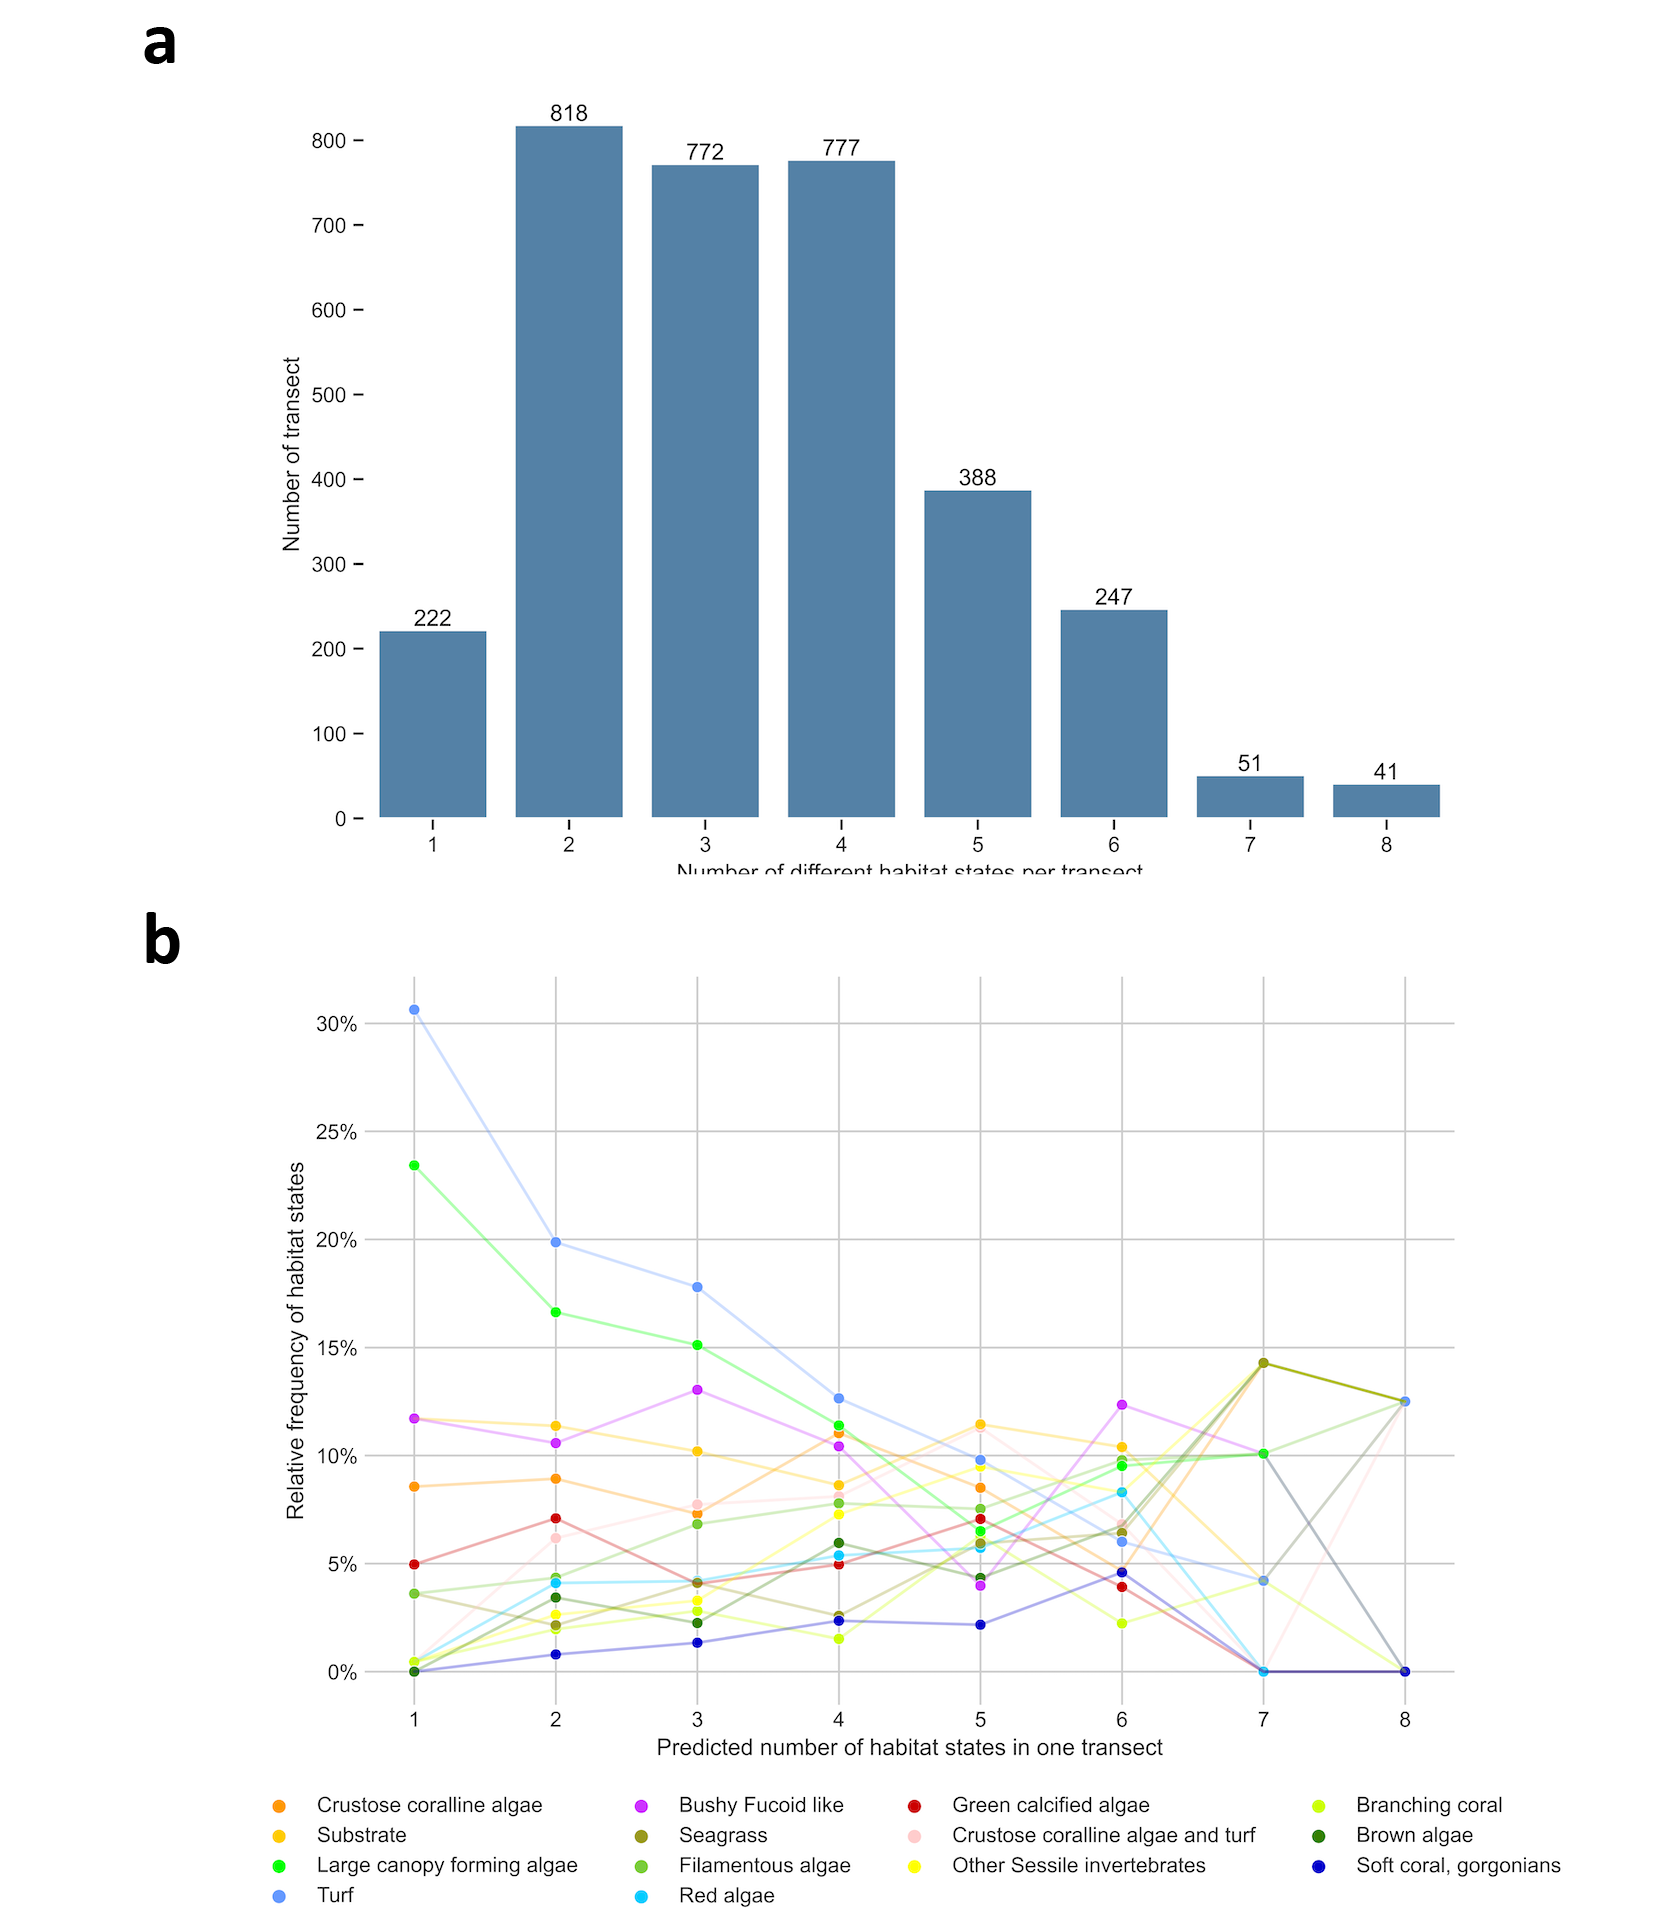
\includegraphics{03-Chapitre3/figures/05-multipanel_fig_ab.png}
\caption{a. Distribution of the number of possible habitat states per
transects, the numbers above the bar represent the number of transects
predicted to have this number of habitat states. b. Relative frequency
of habitat states as a function of predicted number habitat states in
one transect. c.~Heatmap of the frequency of co-occurrence of each
habitat state. Each line of the heatmap has been standardised by the
total number of co-occurrences with the focal habitat
state.}\label{fig:chap3fig3}
}
\end{figure}
\begin{figure}
\ContinuedFloat
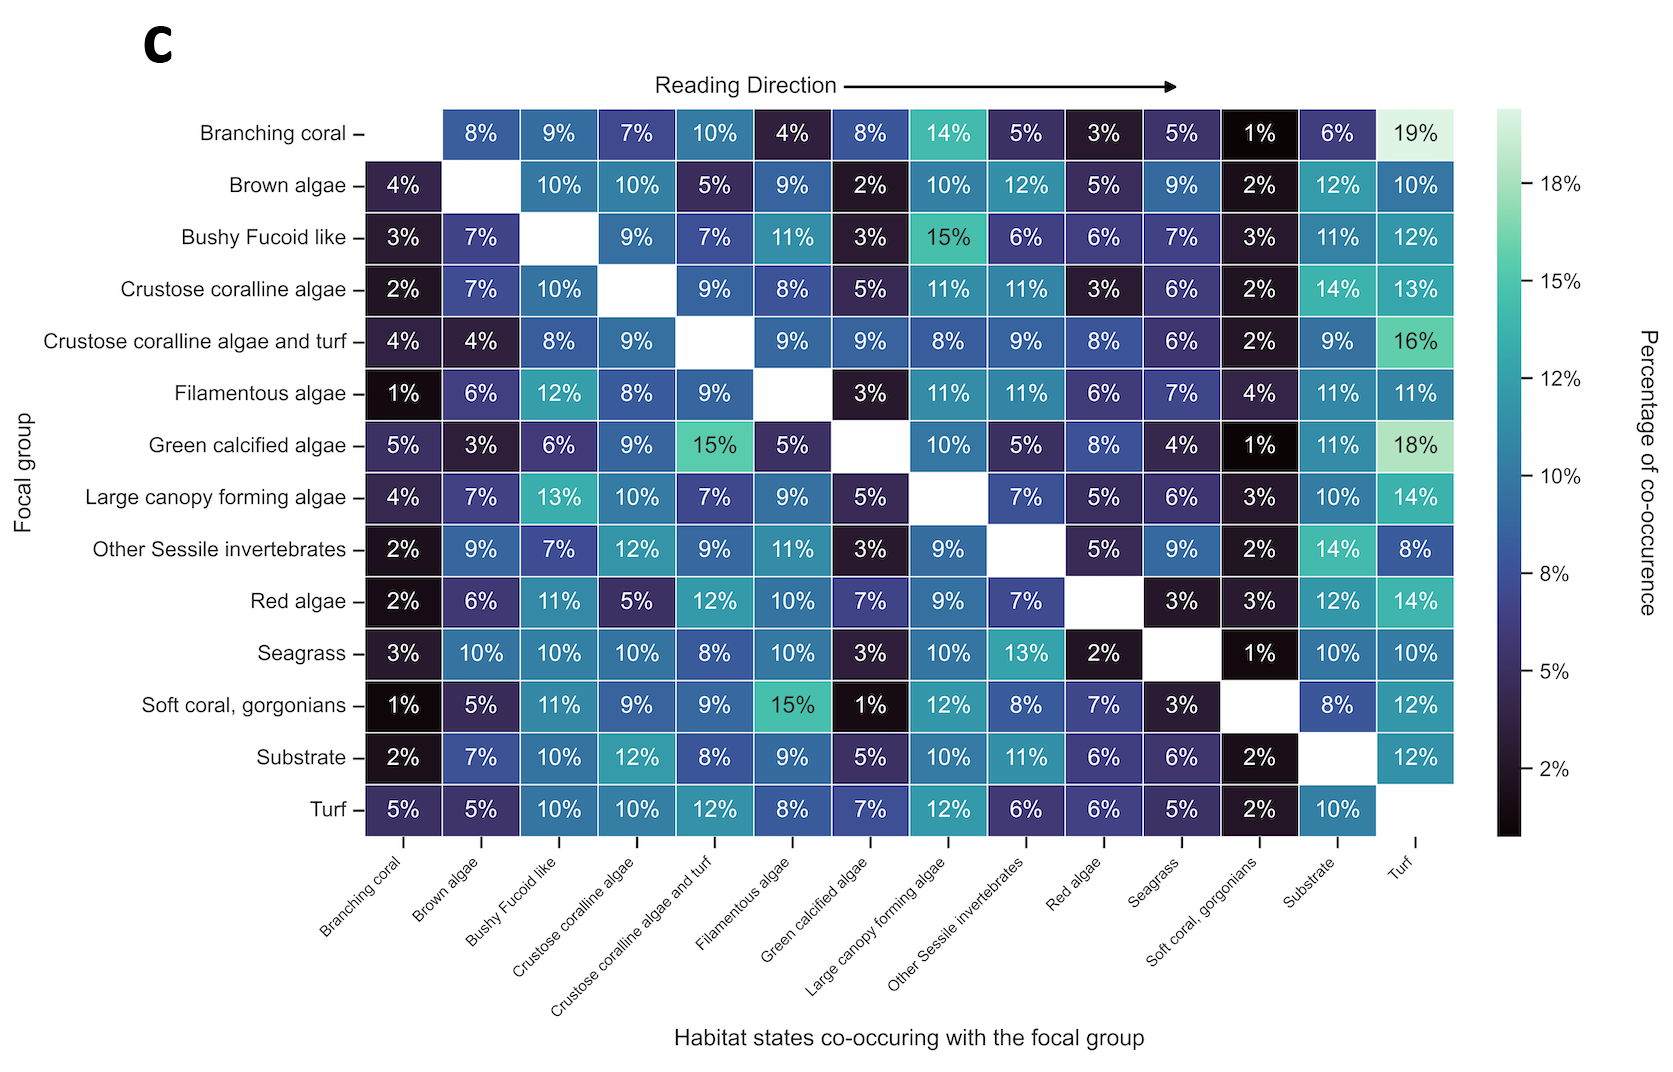
\includegraphics{03-Chapitre3/figures/05-multipanel_fig_c.png}
\caption[]{a. Distribution of the number of possible habitat states per
  transects, the numbers above the bar represent the number of transects
  predicted to have this number of habitat states. b. Relative frequency
  of habitat states as a function of predicted number habitat states in
  one transect. c.~Heatmap of the frequency of co-occurrence of each
  habitat state. Each line of the heatmap has been standardised by the
  total number of co-occurrences with the focal habitat
  state.}
\end{figure}

\hypertarget{spatial-distribution}{%
\subsection{Spatial distribution}\label{spatial-distribution}}

At the Australian geographical scale, different spatial patterns of
richness (i.e.~number of predicted reef states) were observed depending
on the region (Fig.~\ref{fig:chap3fig4}). Most spatial blocks around
Australia have transects where only one unique habitat state can occur
(Fig.~\ref{fig:chap3fig4} a). The majority of spatial blocks have a
median richness of 3 (Fig.~\ref{fig:chap3fig4} b). One has a richness of
6, but the number of transects in this spatial block is relatively low,
with only seven transects sampled. On the east coast of Australia, in
the Tweed-Moreton and Manning-Hawkesbury ecoregions, two ecoregions at
the transition between temperate and tropical zones, the max richness
was 8 whereas the median value of the adjacent temperate or tropical
zones was lower. Over 73\% of spatial blocks can accommodate up to seven
or eight different reef habitat states (Fig.~\ref{fig:chap3fig4} c).
Only the maximum of predicted reef states showed a significant
relationship, albeit weak (linear coefficient of 0.007), with the number
of transects carried out (\(p<0.01\)).

\begin{figure}
\hypertarget{fig:chap3fig4}{%
\centering
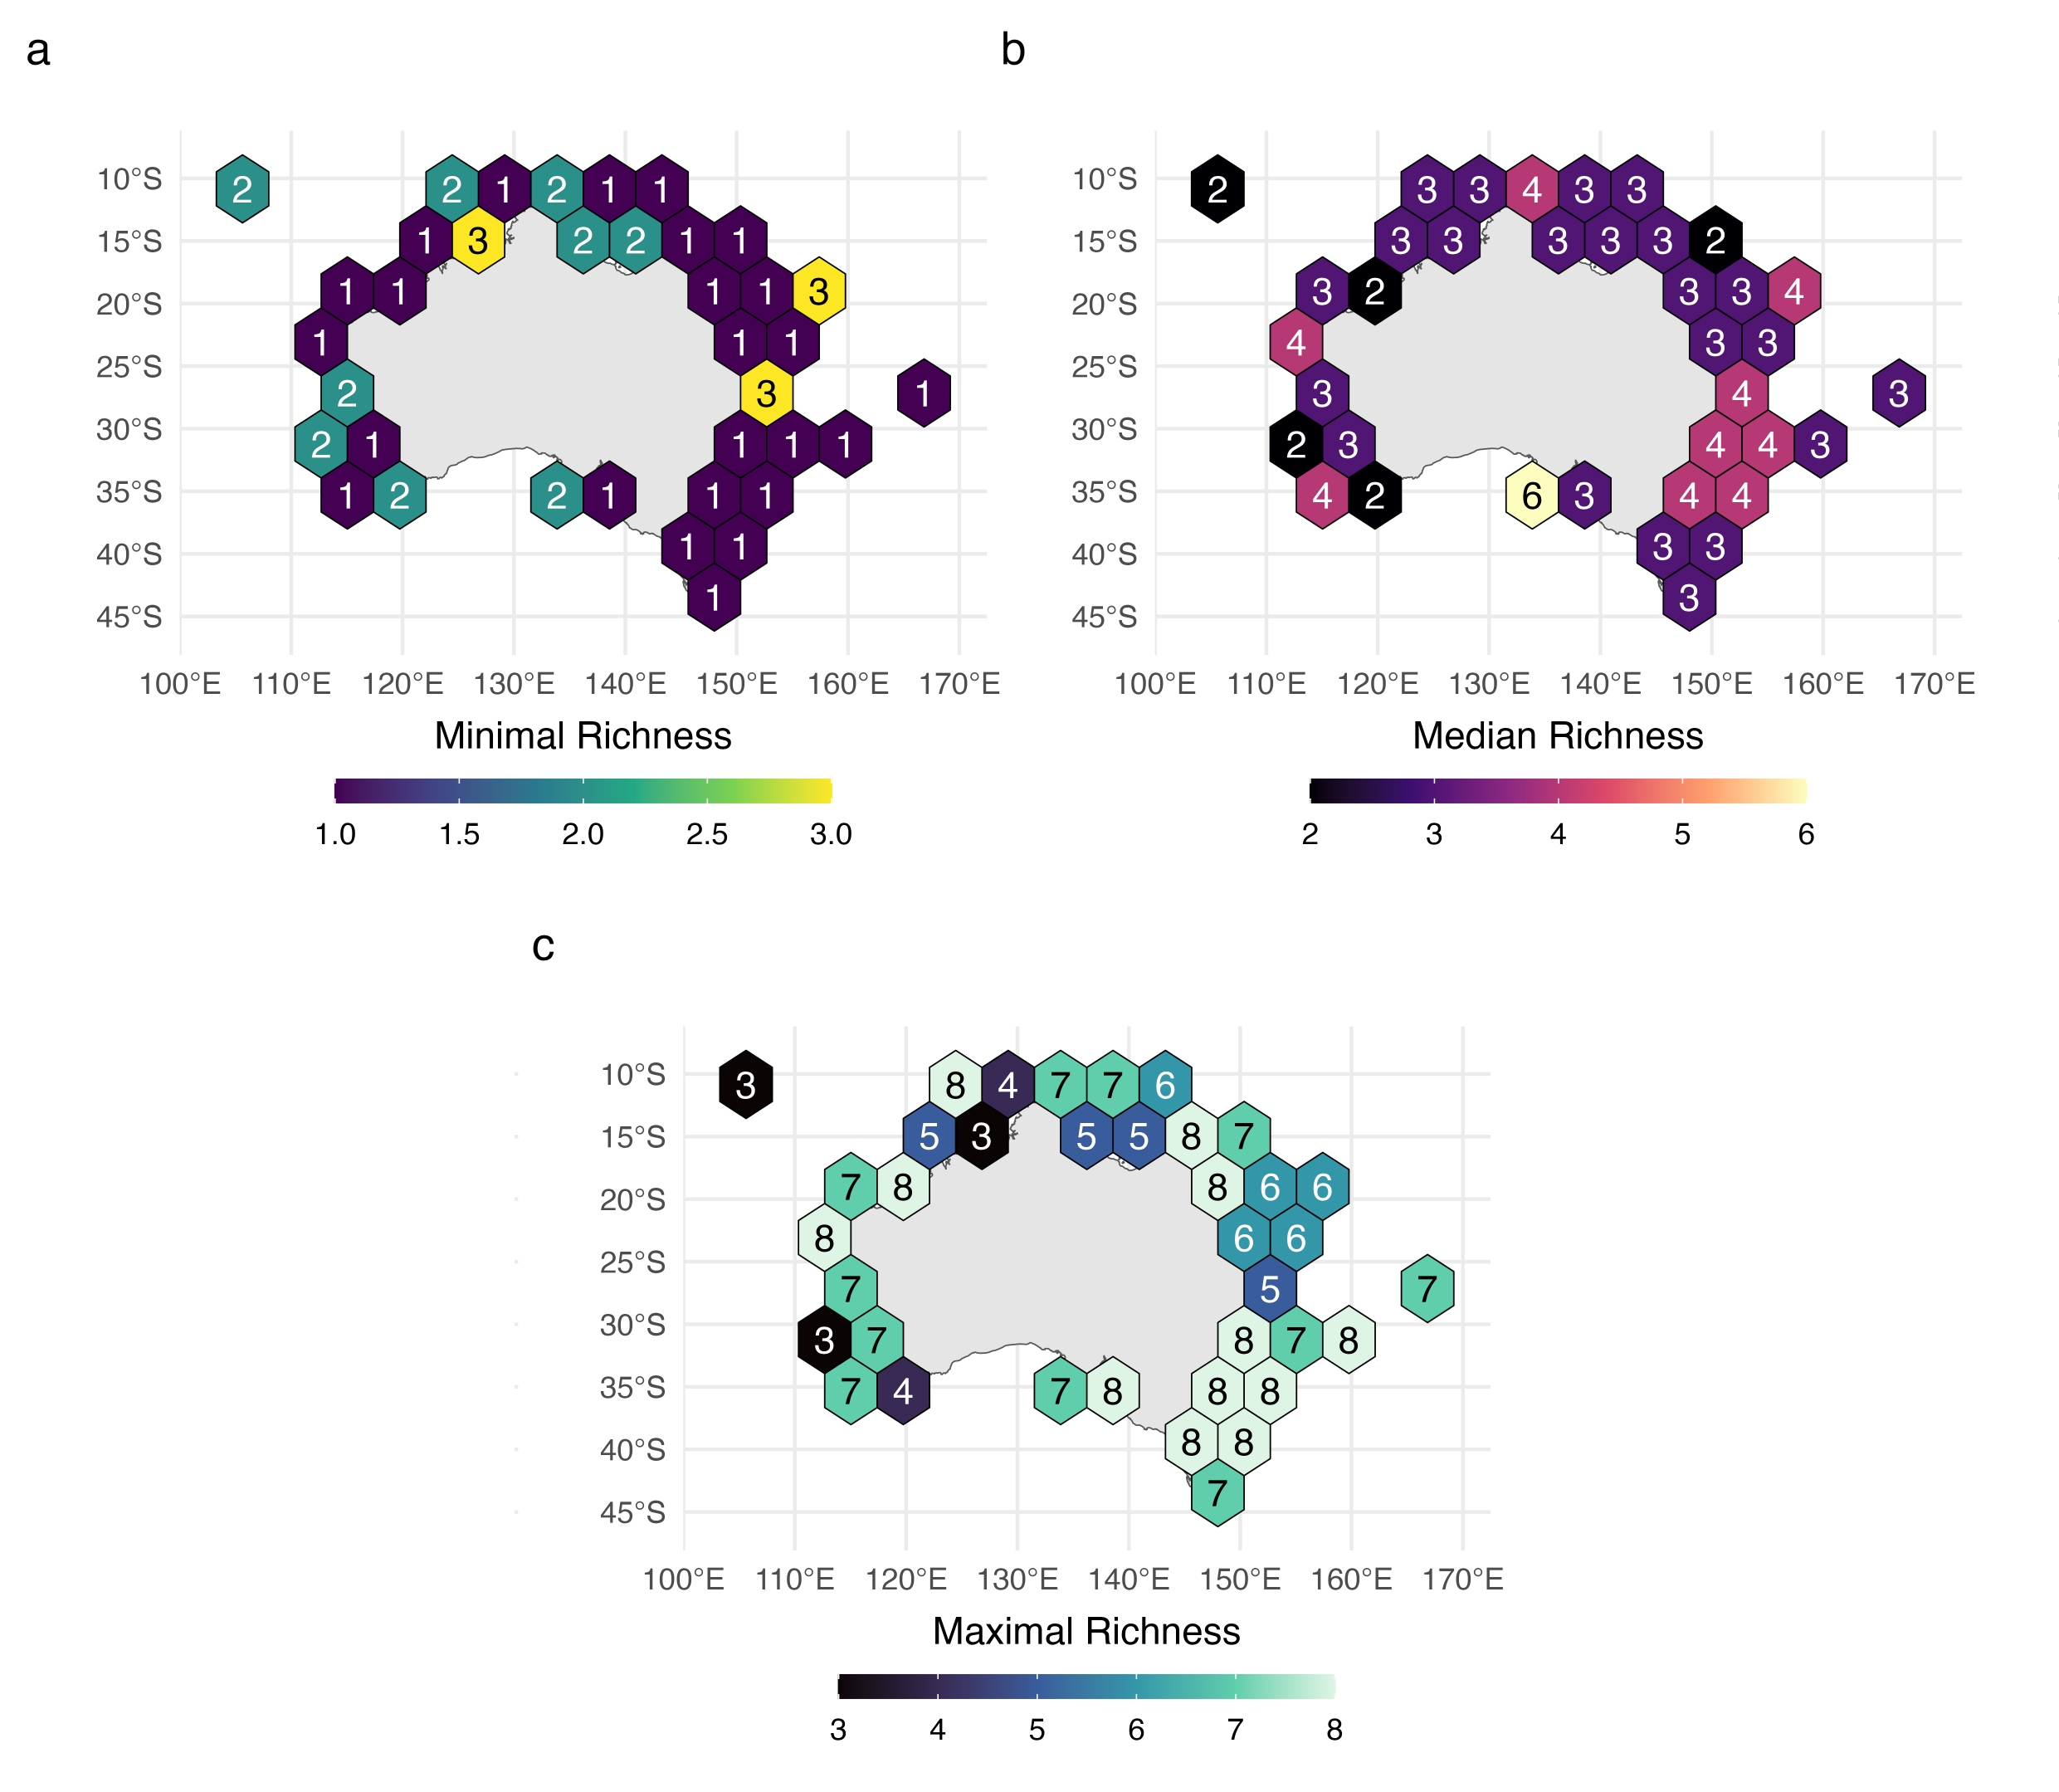
\includegraphics{03-Chapitre3/figures/09-Spatial-block-diversity.png}
\caption{a. Minimal, b. median and c.~maximal richness (i.e.~number of
predicted reef states) per spatial block}\label{fig:chap3fig4}
}
\end{figure}

\clearpage

\hypertarget{discussion-chapt3}{%
\section{Discussion}\label{discussion-chapt3}}

In this study, we built upon Chapter 2 to explain and predict the
spatial distribution of multiple reef benthic habitats. Overall, the
random forest multivariate modelling approach we have used showed
substantial explanatory power but a low predictive power, suggesting
poor transferability. Despite evidence for a good explanatory power, all
predictors presented a similar contribution to the variance explained
precluding us to clearly identify the drivers of the spatial
distribution of most habitats. Partial dependence plots highlighted some
meaningful relationships and showed a differential response of habitats
along environmental gradients that may ultimately trigger the emergence
of alternative stable states. Importantly, some environmental conditions
appeared to be suitable for several habitats suggesting that the current
existence of an habitat in a given area may be due to historical
contingencies and/or biotic settings.

\hypertarget{explanatory-and-predictive-power-of-the-model}{%
\subsection{Explanatory and predictive power of the
model}\label{explanatory-and-predictive-power-of-the-model}}

Our model demonstrates some explanatory power, especially when it comes
to elucidating the distribution of the rarest habitat states in the
dataset such as Branching coral or Soft coral and gorgonians (See Fig.
S1 in appendix A and Fig. S6 in appendix B). This outcome suggests that
the model is able to decipher the reason why habitat states are absent
and gives us insight about the complex relationships between
environmental factors and habitat states. This strongly contrasts with
the model's predictive power, which is quite low overall. Several
factors may contribute to the low transferability of the models. First,
the reef habitat states defined in Chapter 2 are derived from cover data
of about 50 substratum types defined accordingly to the CATAMI benthic
imagery classification scheme (\textcite{Althaus_2015} ; for further
details, see \textcite{Edgar_2020}), merged into 24 functional group.
Hence, the initial reef state categorisation is based on cover data of
morpho-types that does not take into account the identity of the
underlying species. As a result, some reef states may have large
environmental niches in our model while they are in fact driven by
species with much narrower niches and located in different areas. For
example, the diversity of Crustose coralline algae is estimated at
several hundred different species \autocite{Dean_2015,Twist_2019}, which
can be found in both temperate and tropical zones
\autocite{Sissini_2022}. The same goes for Turf, which is a rather
loosely defined functional group \autocite{Connell_2014}. Turf can
include nearly a hundred different species, sometimes with a lack of
consistency in its definition across space \autocite{Connell_2014}.
Hence, while Turf can be found in both tropical and temperate zones, the
underlying species and their ecology may greatly differ across different
areas \autocite{Filbee-Dexter_2018}. Furthermore, it's empirically
observed that benthic assemblages exhibit more reliable and quantifiable
spatial patterns compared to fish assemblages. This distinction has
considerable implications when it comes to delineating appropriate
management zones \autocite{Sandin_2022}.

Furthermore, discrepancies in predictor resolutions and misalignment
with habitat states pose additional hurdles \autocite{Potter_2013}. Our
environmental dataset operates at best at a resolution of 1 km\(^2\),
while the photo quadrats from \emph{RLS} transects, cover an approximate
area of 20 m\(^2\). This spatial disparity hampers the models to make
accurate predictions \autocites[ ]{Connor_2018}{Moudry_2023}, the
estimation of environment-species relationships may be flattenned
\autocite{Meynard_2023}, resulting in an incorrect estimation of
environmental niches. Variability of sampling effort per spatial block
and differences in habitat states prevalence could be another potential
explanatory factor for the model's limited predictive power. Variations
in data collection intensity across different spatial blocks or habitats
could introduce bias and affect the MaxTSS threshold and thus model
prediction performances \autocites[ ]{Somodi_2017}{Leroy_2018}. However,
it is unlikely that our predictive performances were particularly
affected by the choice of metrics, since for the others the predictive
power was also very low. Finaly, prevalence issues in sampling data
hampered our predictive power in two ways. Firstly, The most prevalent
groups are more prevalent by orders of magnitude. Turf, Canopy forming
algae, Fucoid like algae represent respectively 24\%, 17\% and 13\%,
comparatively to Brown algae, Branching coral and Soft cora and
gorgonians that represent only 2\% and 1\% each for the last two in the
whole dataset (Fig. S1).

In light of these challenges, it is important to recognise that while
our model apparently performs well in explaining the distribution of
habitat states, its practical utility for making precise predictions is
rather limited. Nonetheless, there are strategies for enhancing
predictive power, such as improving predictor resolution to be closer to
the scale at which transects are sampled, increasing sampling in the
less well sampled spatial block, or the use of machine learning
techniques to over-sample less prevalent habitats or under-sample more
prevalent ones \autocite{He_2009}. This latter strategy has not been
applied in this study, as it is could be an alternative to the
spatial-block approach that we used in this study \autocite{Gaul_2022}
especially when the data come from a citizen science program \autocites[
]{Robinson_2018}{Robinson_2020}. All the avenues presented here could be
used to improve the predictive power of this type of model, but further
studies are still needed to assess the extent to which each of the
approaches presented, such as upscaling methods (e.g.
\textcite{Meynard_2023}) or over/under-sampling, can improve the
predictive power of \emph{SDMs}.

\hypertarget{influence-of-biophysical-factors-and-anthropogenic-pressures}{%
\subsection{Influence of biophysical factors and anthropogenic
pressures}\label{influence-of-biophysical-factors-and-anthropogenic-pressures}}

The most important variables identified for the different habitat states
were, in order, Sea Surface Temperature, Fishing PC1 and Marine
Heatwaves Anaomaly. Conversely, the variables manifesting the least
influence across all habitat states were anthropogenic pressures,
specifically Nutrient Pollution and Direct Human Disturbance. Our
findings align with those of \textcite{Jouffray_2019}, yet it is crucial
to acknowledge a limitation that both our study and theirs share.
Certain anthropogenic pressures, such as Nutrient Pollution, can be
highly localized, posing challenges for regional models to accurately
capture. Consistent with the observations of \textcite{Jouffray_2019},
our model underscores the critical role of Sea Surface Temperature in
shaping habitat states. This aligns with previous literature emphasizing
temperature's significance in predicting benthic diversity patterns, as
evidenced by \textcite{Belanger_2012}.

Response curves provide insights into the relationships between
environmental factors and certain habitat states. Overall, the response
curves we have generated exhibit a commendable degree of consistency
with the existing literature. For instance, we confirm that Filamentous
algae tend to thrive in areas less exposed to marine currents
\autocite{Quintano_2015}, while Branching coral are more prevalent in
warm temperate waters \autocite{Higuchi_2015}. These patterns provide
valuable ecological insights and corroborate our understanding of the
response of these habitats along environmental gradients. However, it is
important to recognise that not all relationships exhibit such
consistency. Notably, the positive link between fishing pressure or
marine heatwaves and the prevalence of Large canopy forming algae, is
less straightforward and even seems contradictory
\autocite{Wernberg_2016}. It is crucial to contextualise these findings
within the framework of our modelling approach. The SDM model employed
in this study is correlative by essence \autocite{Shabani_2016}, only
capturing statistical associations between environmental variables and
habitat states. While these correlations can reveal important ecological
patterns, they do not establish causal relationships. Understanding the
drivers behind these relationships requires a nuanced perspective. For
example, the observed positive correlation between Large canopy forming
algae and commercial fishing activity may be the result of the high
fishing commercial value of kelp forests, where approximately \$30,000
of fish products are extracted per hectare and per year
\autocite{Eger_2023}. Similarly, the relationship between marine
heatwaves and the probability of occurrence of Large canopy forming
algae should be interpreted in the context of ecological dynamics that
Australian shores recently experienced. Indeed, major episodes of marine
heatwaves occurred in 2011 and 2015 (Hobday et al.~2018) that have led
to the decline of kelp, a common large canopy-forming species, in the
following years \autocite{Wernberg_2016}. This may lead to a spurious
correlation in our dataset, since transect may have been sampled in
these areas before the kelps disappeared. Furthermore, Large Canopy
Forming algae contains more than just temperate macroalgae, some species
of tropical fleshy macroalgae such as Sargassum spp. have been
incorporated as Large canopy forming categories. This kind of fleshy
macroalgue can be found growing on the top of coral reef after a regime
shift to a macroalgae dominated reef \autocite{Smith_2022}, especially
if the coral reef has been degraded due to marine heatwaves
\autocite{Donovan_2021}.

\hypertarget{co-occurrence-patterns}{%
\subsection{Co-occurrence patterns}\label{co-occurrence-patterns}}

Our exploration of co-occurrence patterns among reef habitat states has
yielded intriguing findings shedding light on the ecological dynamics of
these underwater ecosystems. It's striking to note that only a mere 2\%
of the possible combinations among the 14 habitat states were observed
in our data. This limited co-occurrence of habitat states within
transects suggests a complex interplay of ecological factors governing
their distribution. Certain habitat states exhibit weak co-occurrence
patterns with others, implying distinct environmental responses or the
ability for these states to thrive in inhospitable conditions. For
instance, Branching coral and Soft corals and gorgonians rarely co-occur
(Fig.~\ref{fig:chap3fig3} c.), this can be explain by the small number
of corals habitats states in our dataset (see Discussion in Chapter 2).
It can also be a manifestation of niche differences between the two
differents groups, although competition between these two groups may
also contribute to this pattern \autocite{Sammarco_1983}.

Another interesting observation concerns Large canopy forming algae, and
Turf that are frequently predicted alone. While this pattern could be
the result of a bias in our model where the differential prevalence of
habitat states combined with the variable number of transects per
spatial block could influence the joint occurrence probabilities
predicted by the model in each observational unit, an ecological
explanation is also possible. Specifically, we found that other habitat
types presenting similar characteristics with wide ecological niches and
a high prevalence (e.g.~Bushy Fucoid-like, Crustose coralline algae;
Fig. S1 in appendix A) do not exhibit similar patterns
(Fig.~\ref{fig:chap3fig3} b.), this observation suggests that the
influence of the this bias may be less pronounced than initially
perceived, indicating the potential involvement of other underlying
factors. For Turf it may be due to areas that have already undergone a
regime shift (i.e.~the original habitat has disappeared and has been
replaced by Turf; \textcite{Jouffray_2015}), regime shift that struck
hundreds of kilometres of Australian coastline
\autocite{Filbee-Dexter_2018}. For Large canopy forming algae, it may be
due to a bias in the \emph{RLS} sampling method, which, with its
photoquadrat, does not take into account understory habitat, such as Red
algae, Brown algae and Crustose coralline algae, thus underestmating the
niche of the low-profile understory habitat states.

\hypertarget{richness-spatial-patterns}{%
\subsection{Richness Spatial Patterns}\label{richness-spatial-patterns}}

Our examination of spatial richness patterns within spatial-blocks has
unveiled insights into the distribution of habitat states along the
Australian coast. This analysis raises important questions about the
ecological significance of these patterns and their potential
implications for the region's marine ecosystems. One notable observation
is that the majority of spatial-blocks predominantly exhibit a single
ecological status. This phenomenon highlights the prevalence of specific
habitat types in various regions, which can be either desirable, such as
areas characterised by Large canopy forming, Bushy Fucoid like, or
seagrass \autocites[ ]{Coleman_2017}[ ]{Filbee-Dexter_2018}{Janes_2021},
or less desirable, such as those dominated by Turf
\autocite{Filbee-Dexter_2018}. This raises an intriguing question: do
these unique habitat states persist in areas that have remained largely
unaffected by regime shifts, or do they represent remnants of past
ecological transformations? Understanding the historical context and
ecological drivers behind these spatial patterns is crucial to
unravelling their significance.

Intriguingly, the eastern Australian transition zone stands out with a
greater median habitat diversity. This may be linked to the ongoing
process of tropicalisation occurring in the region
\autocite{Figueira_2010}. As the climate warms, there is increasing
evidence of shifts in marine ecosystems, including the expansion of
tropical species into temperate zones \autocite{Verges_2014}. This
phenomenon could potentially lead to regime shifts in the near future
\autocite{Verges_2019}, making the eastern Australian transition zone a
focal point for monitoring and research. Furthermore, it's worth noting
that a substantial number of spatial blocks exhibit the maximum number
of habitat states. This intriguing finding suggests the possibility of
ongoing or impending state changes across the entire Australian coast.

\clearpage

\hypertarget{conclu-chapt3}{%
\section{Conclusion}\label{conclu-chapt3}}

Our study delves into the spatial distribution of multiple reef benthic
habitats and highlighted that some areas are more prone to exhibit
multiple habitat states based on environmental niche similarities. Yet
while our model provides some insights in explaining the distribution of
habitat states and its associated ecological drivers, its predictive
power appeared limited for several reasons including resolution mismatch
between response and predictor variables or the way habitats were
clustered. Despite these limits, which are mostly tailored to the
datasets used, this approach could prove useful to identify the
conditions under which multiple habitats can be found, and therefore the
areas where regime shifts are more likely to take place.

\clearpage

\printbibliography[heading=subbibintoc, title={Bibliographie}]
\end{refsection}